\documentclass[12pt]{mitthesis}
\usepackage{
  lgrind, braket, amsmath, 
  amssymb, bbm, booktabs, 
  subfig
}
\usepackage[pdftex]{graphicx}

\hyphenation{acetylene}

\begin{document}

\subsection*{Electronic Energy Transfer in a Collinear Expansion:\\
  Xe*($^3P_2$) + N$_2$ $\rightarrow$ Xe + 
  N$_2$*(W $^3\Delta_u$, B $^3\Pi_g$, A $^3\Sigma_u^+$)} 

Prof. Ceyer,

An original plan for experiments in our lab was to optically pump
Hg*($^3P_2$) atoms using a two-photon transition and use the
metastable atoms to produce triplet acetylene by collisional energy
transfer during co-expansion in a free jet.  The Hg* and C$_2$H$_2$*
metastables were to be detected by electron ejection from a gold
surface (work function 5.1 eV).

Wilton and I decided to use the Xe* + N$_2$ system as a test case for
acetylene, because the lowest excited state energies for these systems
are well above the work function of gold.  Also, the two-photon
transition to optically pump Xe*($^3P_2$) is at a convenient
wavelength for our lasers.  Additionally, any nitrogen initially
prepared in the B $^3\Pi_g$ state is readily observed by fluorescence
to A $^3\Sigma_u^+$.  The A $^3\Sigma_u^+$ state, in turn, has an
extremely long lifetime, so this technique offers an opportunity to
``preview'' the production of SEELEM-detectable N$_2$* metastables
using fluorescence.

Although we recorded strong signals and made several interesting
observations in both LIF and SEELEM for this system, we decided to
move on to the Hg* + C$_2$H$_2$ reaction; it remained our goal to
obtain new and detailed information on the acetylene triplet states.
However, developments in recent months have renewed our interest in
the Xe* + N$_2$ system.  In this brief note, I'll focus on a
particularly intersting dataset from 2006 and discuss it in light of
our current results.

\subsubsection*{2006 Experiments}

One of the most intriguing observations from our first round of
experiments was the SEELEM time-of-flight spectrum recorded using a
small amount of xenon in a beam of nitrogen (see
figure~\ref{fig:old-tof}).  A transformation of this TOF profile into
velocity space is suggestive of forward-scattered N$_2$* with
vibrational structure.

Figure~\ref{fig:old-velocity} shows the velocity profile corresponding
to the TOF profile in figure~\ref{fig:old-tof}.  In the plots, a
flight distance of 30cm was used to determine the velocity, and the
SEELEM intensities were corrected for the volume of velocity elements
after the transformation.  The large peak with velocity 485 m/s can be
assigned to Xe* with a translational temperature of 14K, as shown in
the top panel.  The smaller peak at 770 m/s can be fit to a velocity
profile of N$_2$ with the same translational temperature, 14K.

We know from other experiments that a neat molecular beam of acetylene
(having the same mass as nitrogen) travels with a mean flow velocity
of approximately 800 m/s in our apparatus.  From experiments with
50:50 mixtures of nitrogen and xenon, we know that the xenon
metastable peak shifts only slightly from its velocity in neat xenon,
which is close to the value presumed here.

Making the somewhat adventurous assumption that the peaks discussed
above correspond to Xe* and N$_2$ moving at their respective mean flow
velocities in the beam, we can convert to a center-of-mass coordinate
system.  Figure~\ref{fig:old-cm} shows a center-of-mass velocity
profile generated with these assumptions.  Potential curve-crossing
models of the Xe*($^3P_2$) + N$_2$ reaction indicate that N$_2$*
molecules formed in $v'=4,3,2$ of the B $^3\Pi_g$ state will accumulate
translational energy as they exit the reaction on the product
potential surfaces (the translational energy arises in a classical
sense from electrostatic repulsion between the product species) [1].

On the figure, bars have been placed at N$_2$ velocities which
correspond to a full conversion of the reaction exothermicity into
forward velocity of the N$_2$ products.  For example, the $v'=4$ level
of the nitrogen B $^3\Pi_g$ state lies 1113 cm$^{-1}$ below the energy
of Xe*($^3P_2$).  For N$_2$* produced in this level, the limiting
forward velocity of the scattered product molecules is 975 m/s
($=\sqrt{2E/m}$).  In this instance, the effect of backscattered Xe*
was not included, so the location of these bars slightly exceeds the
real limit for N$_2$* translational energy.

The center-of-mass transformed profile shows a peak of metastable
intensity that falls off near the $v'=4$ limit for N$_2$*(B $^3\Pi_g$).
This suggests that we may be observing forward-scattered N$_2$
products with vibrational structure.  A similar effect is not present
for the $v'=3,2,1$ levels of this electronic state.  

Another interesting aspect of forward-scattered N$_2$* is that, if an
isotropic distribution of products is assumed, the SEELEM detector
covers a solid angle of less than 0.1\% of the entire area of
scattered products.  Taking this factor into account, the total
intensity of N$_2$* observed in forward scattering may be much
larger than it appears in our profiles.

\subsubsection{2007/08 Experiments}

The major problem with our previous round of experiments was the
possible presence of ions in the SEELEM time-of-flight profiles.  A
N$_2^+$ or Xe$^+$ ion contains internal energy well in excess of that
needed to eject an electron from a gold surface.

In December 2007, Erika Robertson designed and constructed a simple
ion deflector for our chamber.  This deflector consists of two
parallel screens separated by $\sim$2cm and positioned parallel to the
beam.  A low voltage (around 10V) is sufficient to produce a repeatable
TOF profile which we believe is free from ion signal.

The most recent time-of-flight profiles recorded under similar
conditions to the above dataset do not contain any metastable signal
above the limit for N$_2$*(B $^3\Pi_g$), $v'=4$.  Thus, we conclude
that the signal above a laboratory velocity of 1000 m/s in the above
dataset is due to ions.  

Within the N$_2$ peak observed in the present datasets, there may also
be some structure related to close-lying vibrational levels of the W
$^3\Delta_u$ and A $^3\Sigma_u^+$ electronic states.  This is
presently under investigation by my colleagues.

-- Kyle (March 2008)

\vspace{2cm}

[1] Ch. Ottinger, A.F. Vilesov, and D.D. Xu. \emph{Chemical Physics}
\textbf{192}, 49 (1995).

\begin{figure}
  \caption{Vibrational energy levels and potential curves for N$_2$* W
    $^3\Delta_u$, B $^3\Pi_g$, and A $^3\Sigma_u^+$.  The x-axis is
    the radius of separation between the nitrogen atoms in N$_2$, in
    units of Angstroms.  The y-axis is potential energy in electron
    volts.  The W $^3\Delta_u$ and A $^3\Sigma_u^+$ states of nitrogen are
    metastable, while the B $^3\Pi_g$ state decays by fluorescence to
    A $^3\Sigma_u^+$, with an average lifetime of several $\mu$s.
    Also shown in the figure is the metastable $^3P_2$ level of Xe,
    which lies close in energy to the $v=5$ level of N$_2$* B
    $^3\Pi_g$, the $v=5$ level of W $^3\Delta_u$, and the $v=14$ level
    of A $^3\Sigma_u^+$.  From Kr\"{u}mpelmann, T. PhD Dissertation,
    MPI f\"{u}r Str\"{o}mungsforschung, G\"{o}ttingen (1987).}
  \label{fig:n2curves}
  \centering
  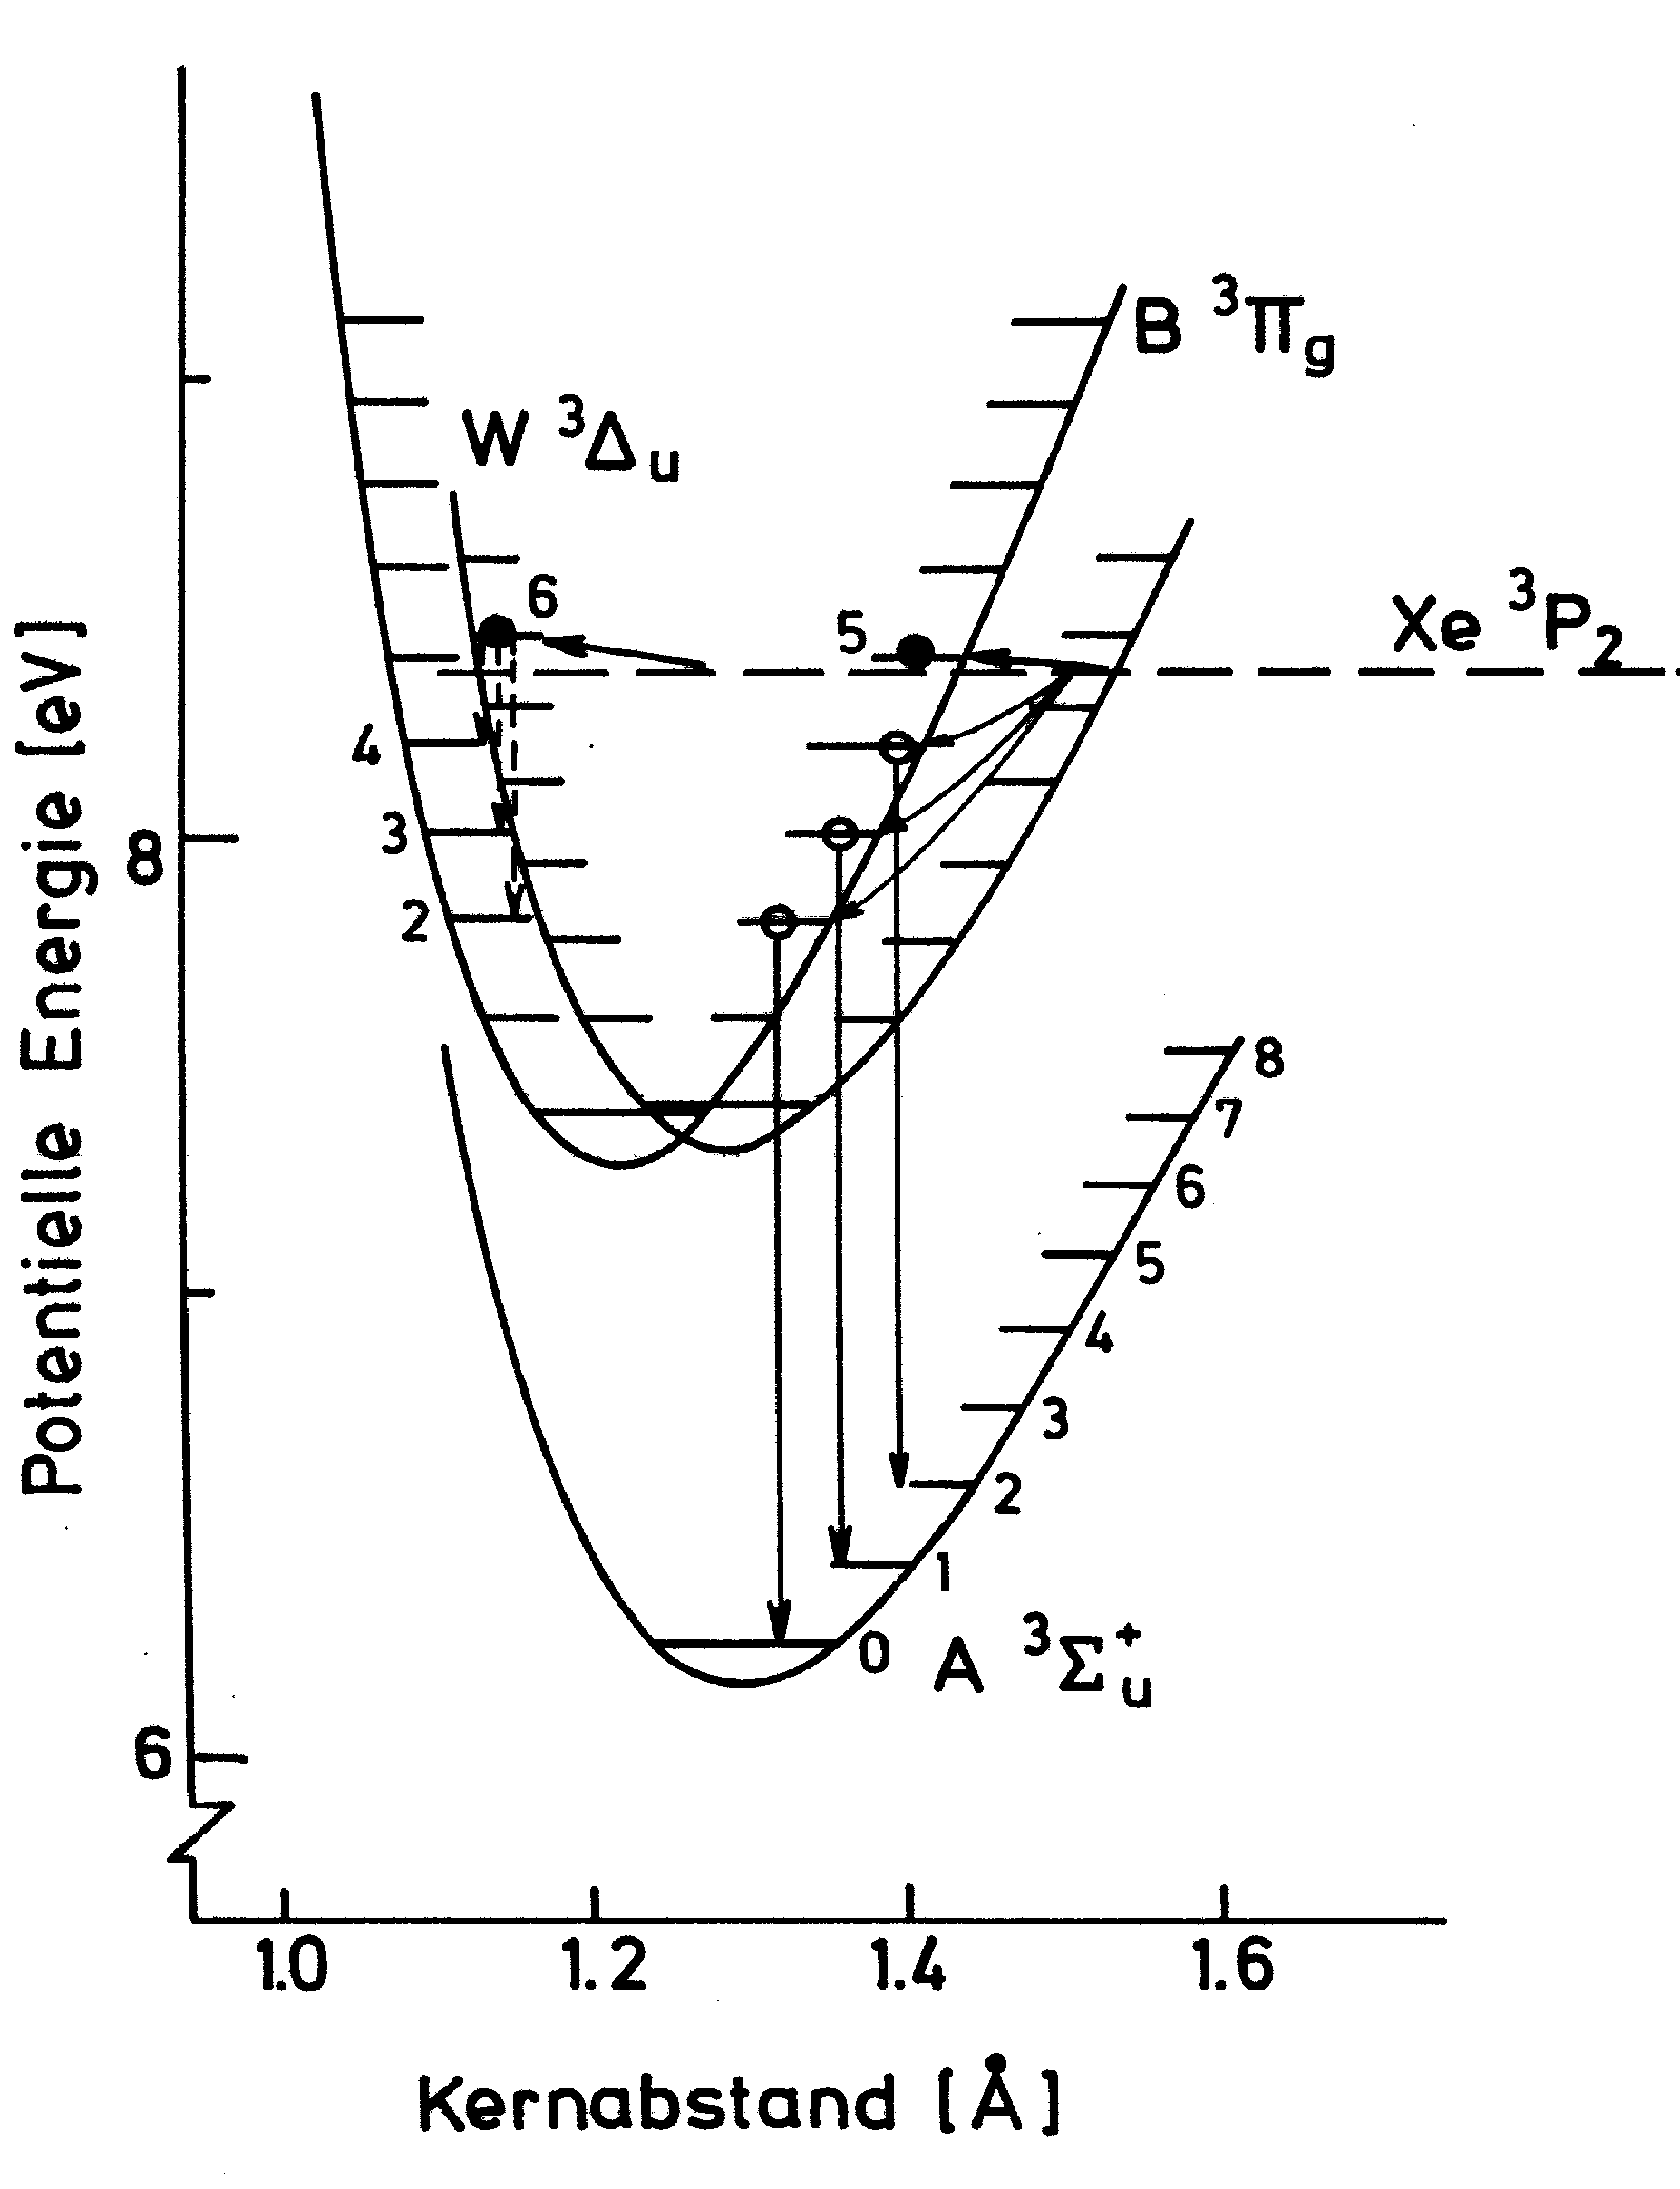
\includegraphics[width=5in]{n2curves.png}
\end{figure}

\begin{figure}
  \caption{Time-of-flight arrival of Xe* and N$_2$* metastables
    detected by SEELEM.  The gas mixture is mostly nitrogen
    ($P_b=24\,psi$), with residual xenon left in the nozzle from a
    previous experiment.}
  \label{fig:old-tof}
  \centering
  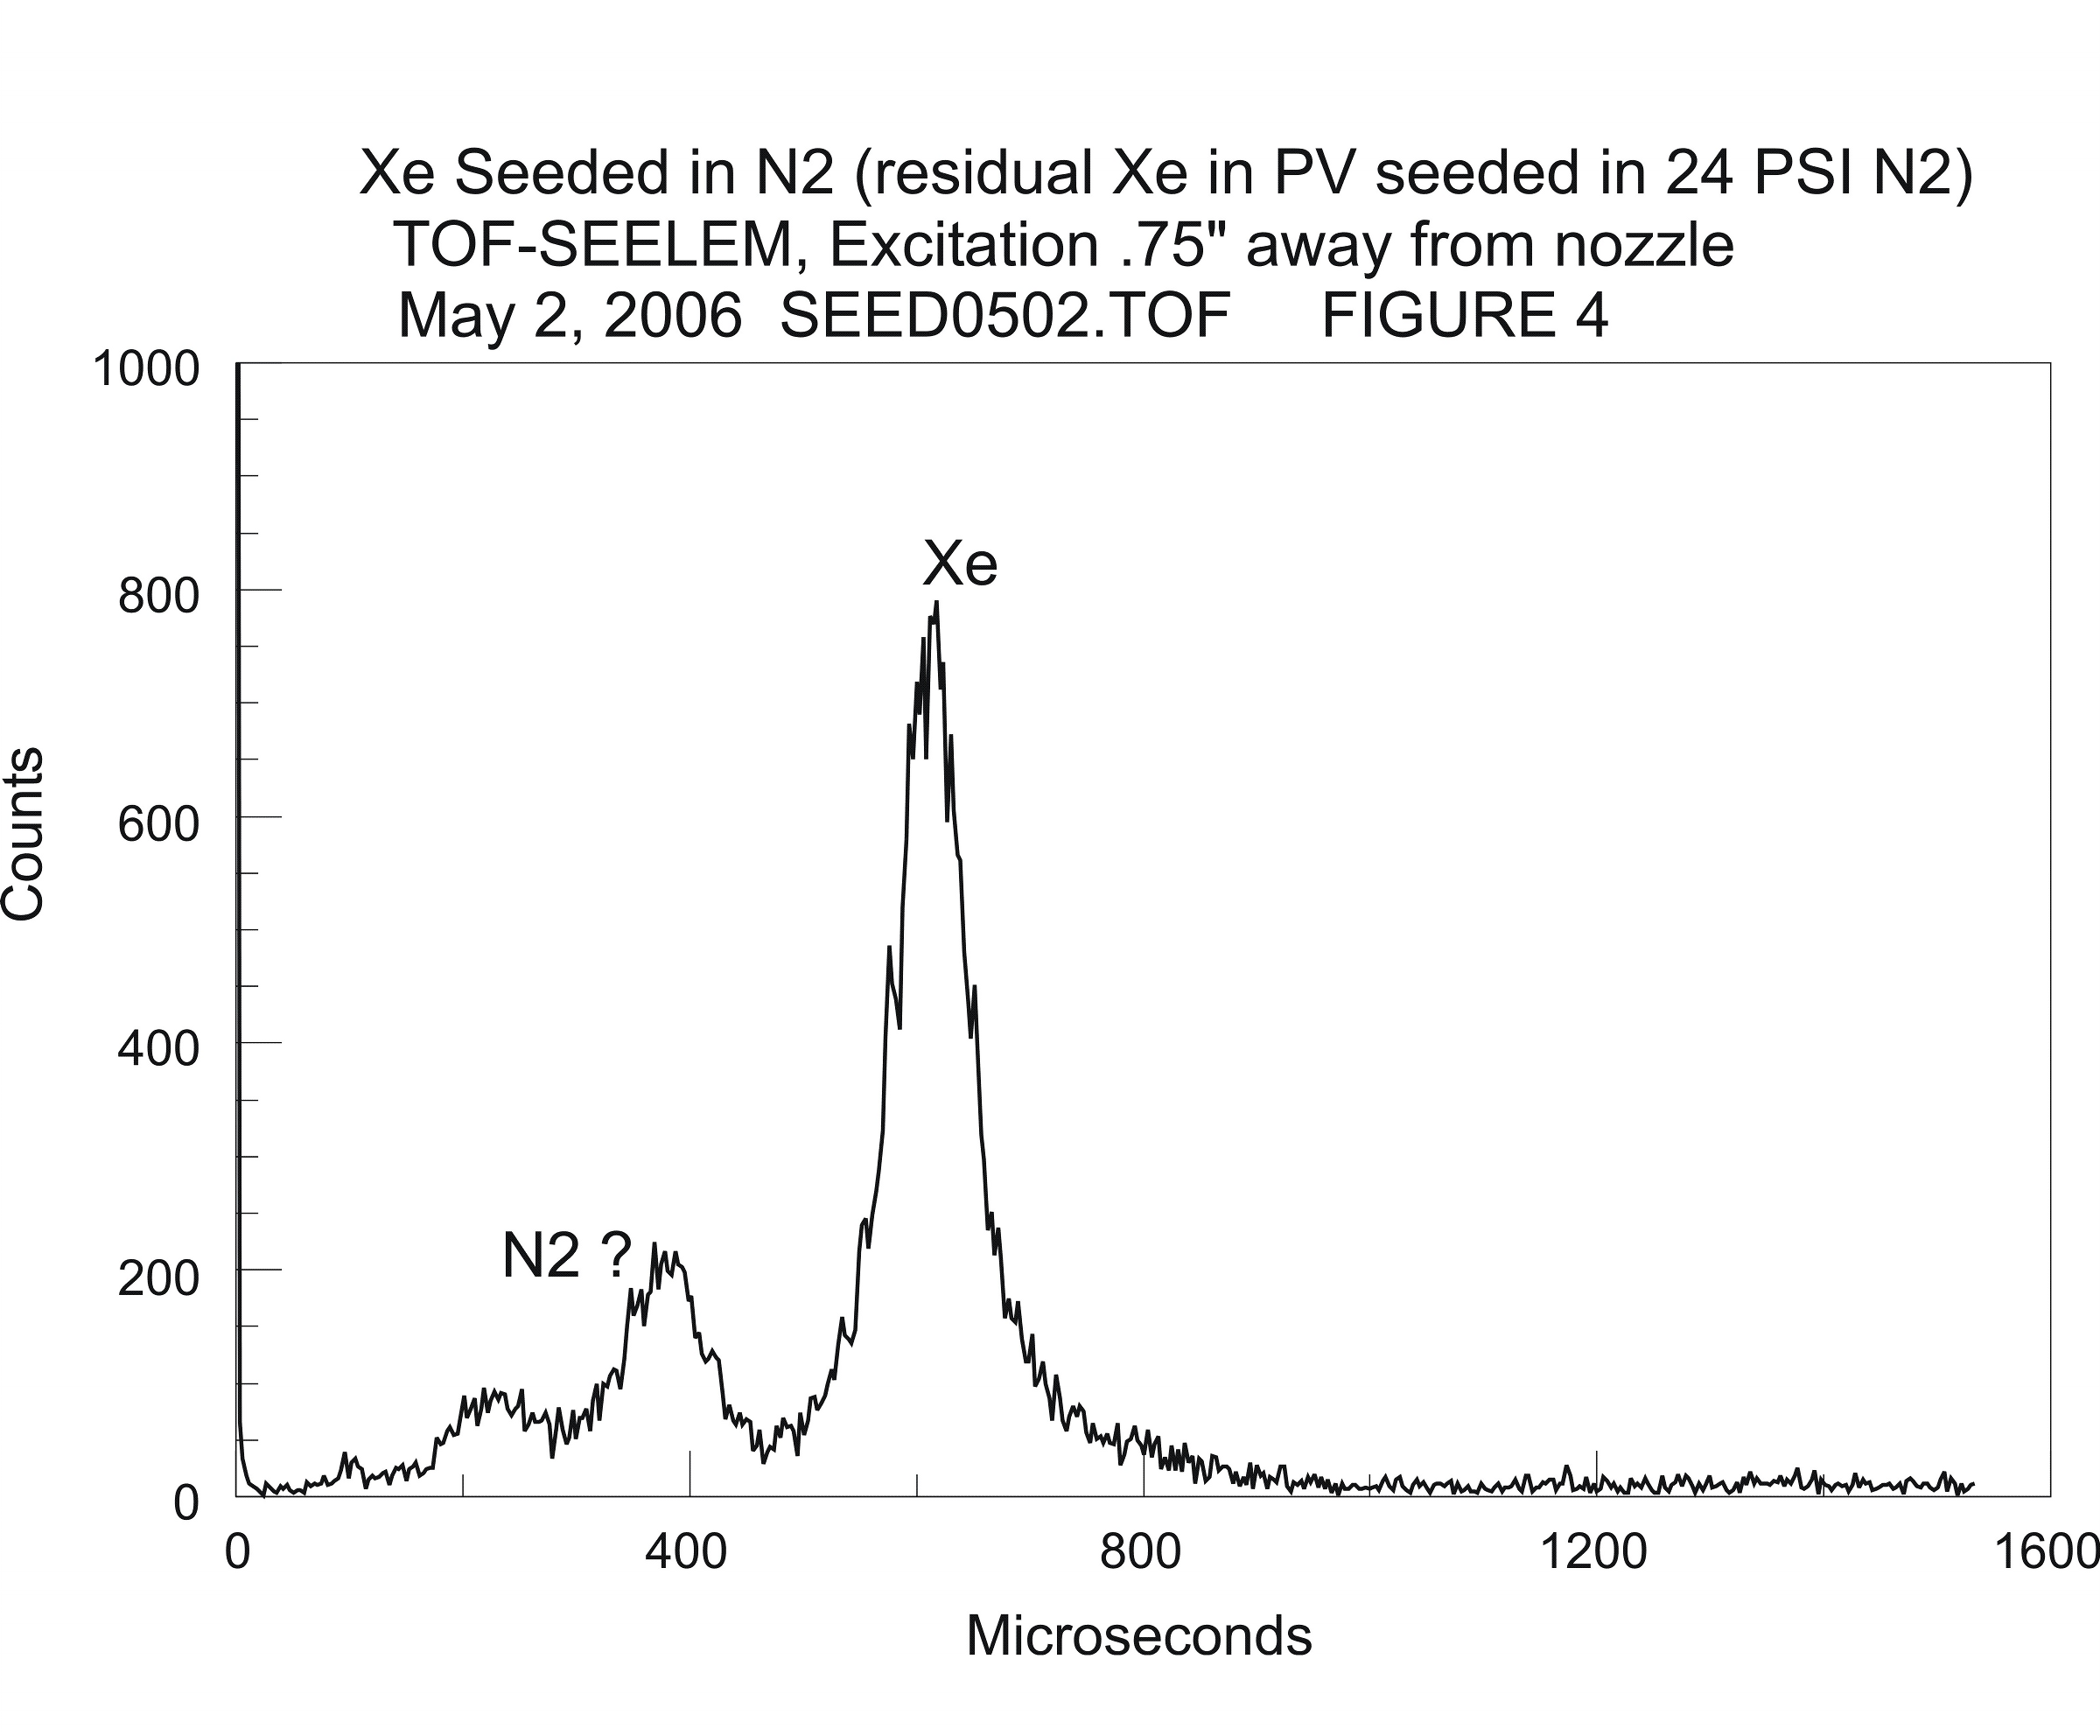
\includegraphics[width=6in]{old-tof.png}
\end{figure}

\begin{figure}
  \caption{Laboratory-frame velocity profiles of Xe* and N$_2$*
    metastables detected by SEELEM, transformed from the data in
    figure~\ref{fig:old-tof}.  The experimental data in both plots is
    identical.  The top plot is overlayed with a velocity distribution
    of Xe atoms having a translational temperature of 14K and a mean
    velocity of 485 m/s.  The bottom plot is overlayed with a velocity
    distribution of N$_2$ molecules having the same temperature and a
    mean velocity of 770 m/s.}
  \label{fig:old-velocity}
  \centering
  \subfloat{
    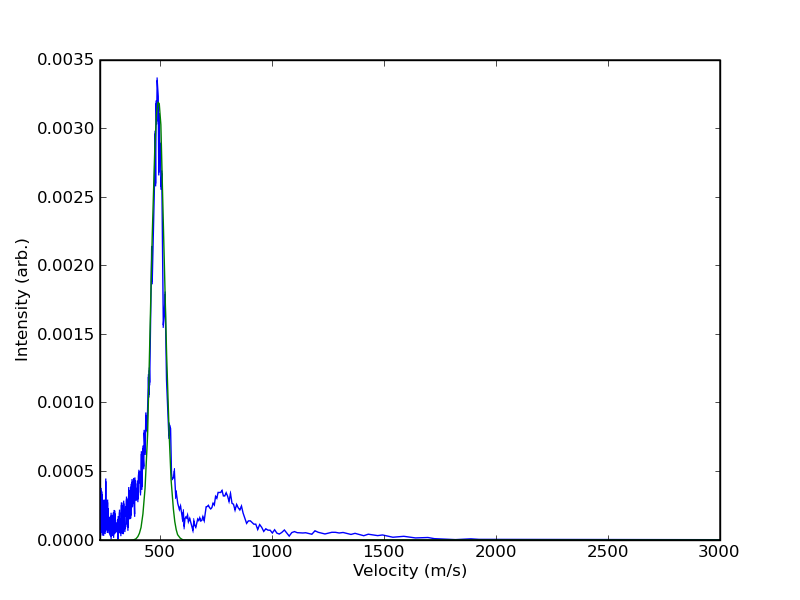
\includegraphics[width=5in]{old-velocity-xe.png}
  }
  \subfloat{
    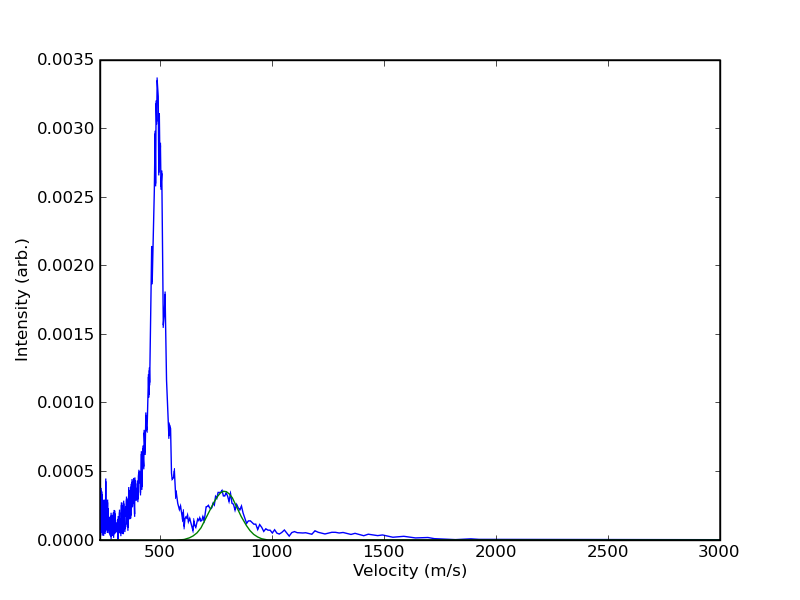
\includegraphics[width=5in]{old-velocity-n2.png}
  }
\end{figure}

\begin{figure}
  \caption{Center-of-mass velocity profile of metastable species
    produced by collisional excitation transfer between Xe*($^3P_2$)
    and N$_2$ after co-expansion in a free jet.  The plot is marked
    with bars that indicate the limit of forward-scattering velocity
    for N$_2$ in the $v=4,3$ levels of the B $^3\Pi_g$ state.}
  \label{fig:old-cm}
  \centering
  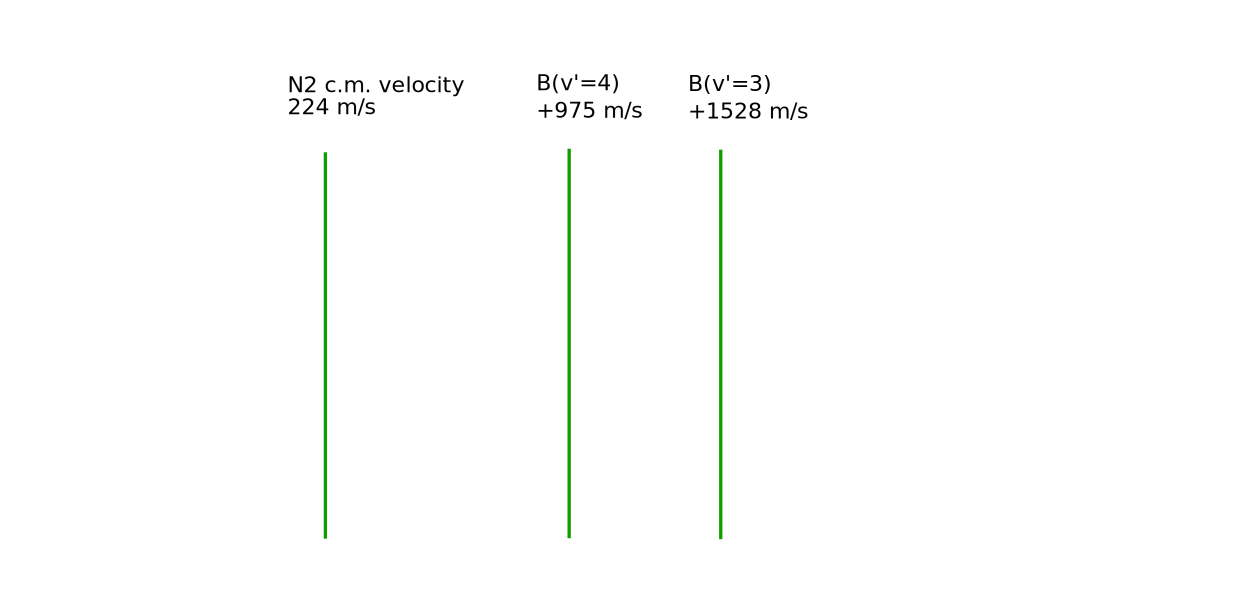
\includegraphics[width=6.5in]{old-cm.png}
\end{figure}

\end{document}